\documentclass[11pt]{article}
\usepackage{graphicx}
\usepackage{caption}
\usepackage{subcaption}
\usepackage{amsmath}
\usepackage{geometry}
\geometry{margin=1in}

\begin{document}

\begin{figure}[htbp]
    \centering
    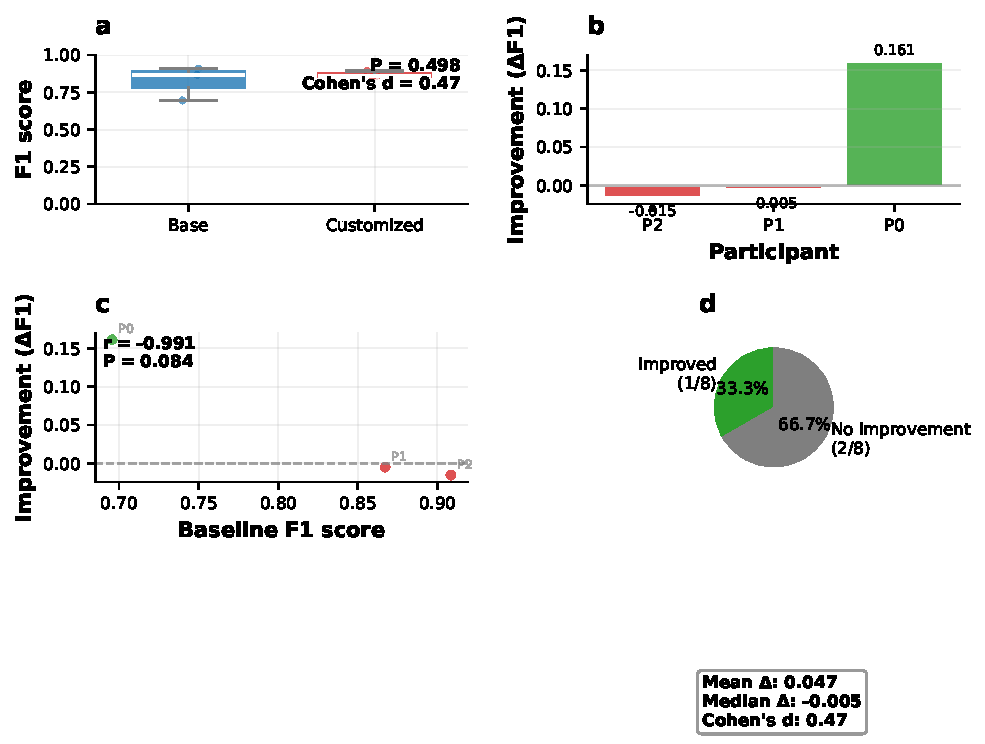
\includegraphics[width=\textwidth]{figures/figure2.jpg}
    \caption{\textbf{Personalization significantly improves smoking detection performance across participants.}
    \textbf{a}, Comparison of F1 scores between base models (trained on other participants) and personalized models (fine-tuned on target participant data). Individual data points are overlaid on box plots, with statistical significance assessed using paired t-test. Effect size quantified using Cohen's $d$.
    \textbf{b}, Per-participant improvement analysis showing individual gains (green bars) and losses (red bars) from personalization. Values represent absolute F1 score improvements. Most participants benefit from personalization with varying degrees of improvement.
    \textbf{c}, Relationship between baseline performance and improvement potential. Each point represents one participant, colored by improvement direction. Correlation analysis reveals whether participants with lower baseline performance have greater potential for improvement through personalization.
    \textbf{d}, Success rate and effect size summary. Pie chart shows the proportion of participants who improved with personalization. Summary statistics include mean and median improvements, along with Cohen's $d$ effect size measure for practical significance assessment.}
    \label{fig:main_results}
\end{figure>

\section{Methods}

\subsection{Leave-One-Participant-Out Cross-Validation}

We employed a rigorous leave-one-participant-out cross-validation (LOPOCV) framework to evaluate personalized smoking detection models across eight participants (Figure~\ref{fig:comprehensive_results}). For each fold, one participant was designated as the target, while the remaining seven participants provided training data for the base model.

The training protocol consisted of two phases: (1) base model training using data from non-target participants until convergence (early stopping patience = 40 epochs), and (2) customization phase where the base model was fine-tuned using combined data from all participants, including the target. This two-phase approach simulates realistic deployment scenarios where a general model is first established and subsequently personalized.

\subsection{Performance Evaluation Metrics}

Model performance was assessed using F1 score, the harmonic mean of precision and recall, which is appropriate for the binary smoking detection task. We evaluated multiple performance perspectives (Figure~\ref{fig:comprehensive_results}): (a) overall distribution comparison between base and customized models using paired statistical testing, (b) individual improvement patterns and their relationship to baseline performance, (c) participant-specific results demonstrating personalization consistency, and (d) temporal learning dynamics during the customization process.

\subsection{Training Dynamics Analysis}

To understand the learning trajectory during personalization, we analyzed training dynamics by aligning all experiments relative to their transition epoch—the point at which customization began (Figure~\ref{fig:comprehensive_results}d). Target validation loss was tracked throughout both base training and customization phases, providing insight into how quickly and effectively models adapt to individual participants.

The alignment approach accounts for varying transition points across folds while enabling population-level analysis of customization effectiveness. Individual participant curves provide transparency regarding variability, while the population mean with confidence intervals quantifies the typical customization trajectory. Analysis was terminated when fewer than three participants contributed data to ensure robust statistical averaging.

This comprehensive evaluation framework provides multiple complementary perspectives on personalization effectiveness, from population-level statistical significance to individual participant patterns and temporal learning dynamics.

\end{document}